\part{Selection and evolution of antibiotic producers in microdroplets }
\chapter{Introduction}
\label{chap:droplets_intro}

This chapter introduces the relevant background and previous research around antibiotic evolution, focusing on antibiotic resistance as a global public-health concern and previous efforts to evolve antibiotic producing bacteria as well as providing reasoning, why structured environments are necessary and well-mixed, liquid environments are not suitable. Furthermore, a section focuses on water-in-oil microdroplets and current technical advancements in this field. The last section describes the research objectives of this project.

\section{Antibiotic resistance is a key threat in public health}

In the last decades, rapidly evolving antibiotic resistance became an increasingly important risk factor in hospital settings and later also in community environments~\cite{David2010-az}. Many efforts have been made to circumvent antibiotic resistance by optimizing treatment regimes~\cite{Kim2014-lq}, re purposing old antibiotics~\cite{Kim2019-qk} or developing entirely new drugs~\cite{Lin2017-sh} but nonetheless antibiotic resistances to clinically relevant antibiotics are commonly found~\cite{Jernigan2020-ro}. We aim to find new ways of overcoming antibiotic resistance by evolving antibiotic producers, while specifically selecting for the increased killing of resistant bacteria.

\section{Antibiotic production in natural communities}
\label{sec:natural_production}

Natural microbial communities often include antibiotic producers which gain a growth advantage over their neighboring cells by producing antimicrobial compounds. These antibiotics may give the producer a fitness advantage as they kill or inhibit the growth of its competitors in the community, often allowing the producers to use components of lysed cells as additional nutrients.
As production of an antibiotic is metabolically costly, a producer gains an advantage over neighboring cells if two criteria are fulfilled:
\begin{enumerate}
\item The concentration of the antibiotic is high enough to kill or inhibit the growth of the surrounding competitors.
\item The benefit from killing or inhibiting growth is high enough to outcompete resistant, non-producing cells, which we also call cheaters.
\end{enumerate}
As cheaters are not affected by the produced antibiotic but also do not produce the specific antimicrobial compounds, they may have a growth advantage over the producer and can thus overtake the free space generated by the producer ("cheating") limiting its fitness advantage.
Resistance can be conferred through evolution e.g. by modifying the receptors where the toxic molecules bind to or by gene transfer of immunity genes as is the case for the well studied colicin toxin in \textit{E. coli}~\cite{Redericq2008-bn}.
A long-term goal in antibiotic research is the challenge of finding conditions in which bacteria evolve to produce novel antibiotics or towards modifying existing ones, effectively emulating such natural communities~\cite{Charusanti2012-uy}.

\section{Selection is not possible in well-mixed environments}

The effect of an antimicrobial compound in spatially structured environments is limited by diffusion to the immediate surrounding of the producers. Consequently, growth inhibition occurs only in close proximity to a colony of producers. One could think, that the use of a well-mixed environment could increase the effect of the antibiotic.
However, due to constant mixing in a well-mixed environment, the antibiotic produced is usually dispersed throughout the culture and does not accumulate to a high enough concentration required to actually kill competitors, as sketched (not to scale) in figure~\ref{fig:intro_droplets_idea}a. Moreover, even if the antibiotic accumulates to a concentration high enough to kill competitors (due to high production rates or a large number of producing cells), the chance of an existing cheater growing equally fast or even faster than the producer is close to 1.
Hence, according to the criteria defined in Section~\ref{sec:natural_production}, producers do not have a growth advantage over other cells in well-mixed environments and are usually not selected for or are even outcompeted by cheaters due to the significantly lower growth rate as a result of antibiotic production.

\section{Spatial structures enable selection for antibiotic producers}
\label{sec:spatial_structure}

Agar plates as spatially structured environments were used in a previous study in our laboratory to show that producers have a growth advantage compared to cheaters when grown in competition with sensitive cells (the colonies of producers are bigger than the ones of cheaters). However, as soon as a cheater is in close proximity to a producer (within the inhibition zone of the latter one), it will profit from the killing of the sensitive cells. Hence, one can only work with very low producer densities on agar plates to minimize the probability that a cheater is in the inhibition zone created by a producer~\cite{Gerardin2016-ac}. The small population size available in this setting limits the potential for de novo mutations, which would lead to evolution of the antibiotic producer.

\begin{figure}
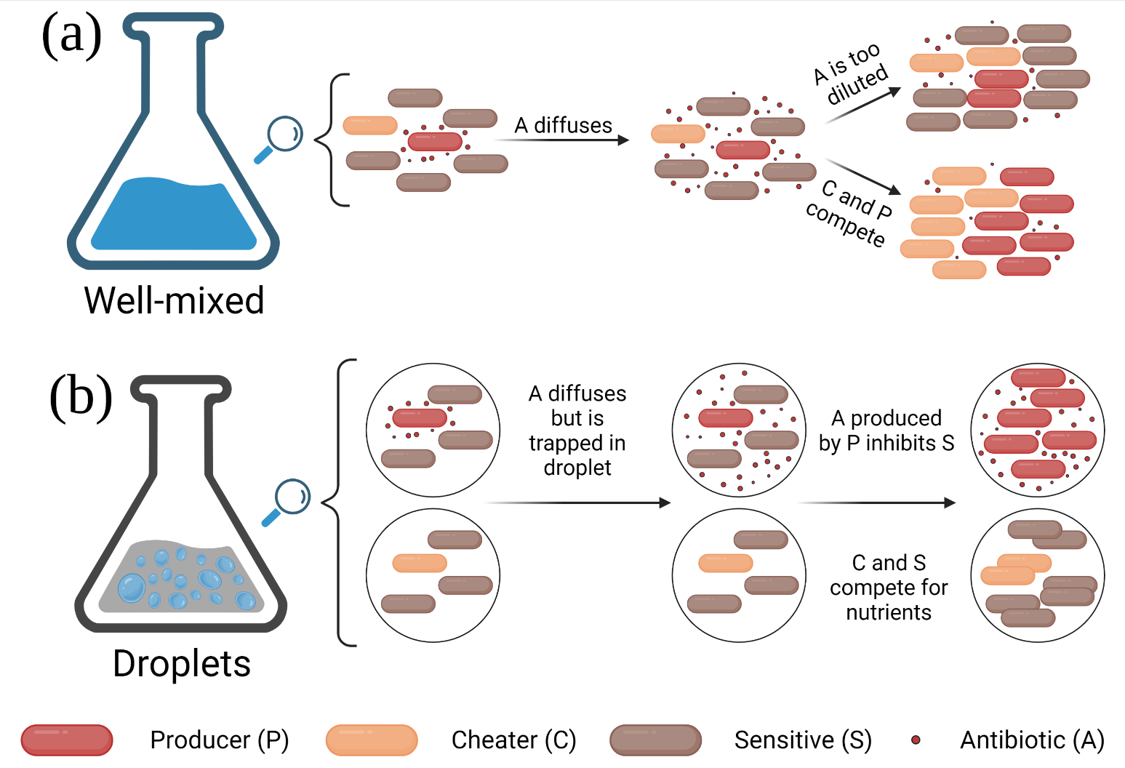
\includegraphics[width=\linewidth]{graphics/2025_09_30_droplets_fig1.png}

\caption{\textbf{Microdroplets provide a platform for selection of antibiotic producing cells.} In this sketch, the interactions between sensitive (brown), producing (red) and cheating (orange) cells in a well-mixed (a) and in a water-in-oil droplet (b) environment are shown. \textbf{(a)} Upon production of the antibiotic (red particles), it is immediately dispersed through the entire culture due to constant mixing. Two possible outcomes are possible, as sketched here. In the first outcome, the antibiotic is too diluted to inhibit growth (as shown in the upper part) and all cells grow at a similar rate. In the second outcome, the antibiotic is highly concentrated and kills the sensitive cells in the entire culture as shown in the lower part. Due to the killing of all sensitive cells, the cheater cells can equally profit from the absence of the sensitive cells and both, producers and cheaters, grow. \textbf{(b)} In droplets, producers and cheaters can be separated in different droplets as depicted here. The producer will target sensitive cells trapped in the same droplet as the produced antibiotic molecules cannot disperse through the entire culture (into other droplets). So the producer is the only cell which profits from the effect of the antibiotic and grows faster than cheaters and sensitive cells in competition in other droplets as depicted in the last step.}
\label{fig:intro_droplets_idea}
\end{figure}

\section{Water-in-oil microdroplets as a technology for high-throughput spatially structured microenvironments}

In recent years, microdroplets have become a commonly used technology in biomedical applications~\cite{Zagnoni2011-ko}. They enable us to encapsulate small volumes $ \left( \approx 50 \mathrm{pl} \right)$ of growth medium and competing cells in separate microenvironments as sketched in figure \ref{fig:intro_droplets_idea}b. Due to the high generating frequency in microfluidic chips, currently accessible $\left( \approx 10^4 \frac{\mathrm{droplets}}{\mathrm{s}} \right) $, we can now perform high-throughput experiments.
Therefore, with microdroplets, we can replace the problem mentioned in Section~\ref{sec:spatial_structure} of a limiting density of producers on agar plates with the problem of a limiting concentration of producers in the aqueous phase which can more easily be dealt with by producing more droplets, which is a matter of time rather than a matter of space as it was on agar plates~\cite{Gerardin2016-ac}. Having longer production times for droplets would increase the number of produced droplets by up to $10^4$ droplets per second.
Assuming the chance for a mutation which modifies antibiotic production to be $10^{-8}$~\cite{Drake1998-es, Kunkel2004-br, Wielgoss2011-jd} and our ability to easily reach $10^7$ droplets in a reasonable time, we can considerably increase the chance of obtaining such mutations compared to agar plates used previously, where the maximal number of distinct colonies reached $10^3$~\cite{Gerardin2016-ac}.

\section{Objectives of the project}

The project has three main objectives:
\begin{enumerate}
    \item We try to establish a high-throughput microdroplet system to select for antibiotic producing cells.
    \item We try to select for the antibiotic producing cells in competition with sensitive and cheater cells in microdroplets.
    \item We want to find evolutionary pathways leading to de-novo mutations within the antibiotic producing cells which help overcoming evolved resistance.
\end{enumerate}
By evolving the antibiotic to target resistant cells, we would be able to isolate the antibiotic from its producer in a next step as done before~\cite{Singh2018-qp} and one could conduct clinical studies to use this antibiotic in patients treatment. The project could serve as a proof-of-principle how one could try to target the increasing threat of antibiotic resistances.
The resulting mutations could offer a general way to improve antibiotics effectiveness which is not known yet and could lead to new opportunities of generating new, enhanced antibiotics which can be used to treat infections with resistant bacterial strains.
Unfortunately, the chosen biological system (antibiotic producer and sensitive target strain) was not ideal and especially the antibiotic producer did neither grow in droplets nor produced the expected antibiotic in a standard liquid culture. Nevertheless, we were able to achieve the first objective of the project.

